\appendix

\zsavepos{header-1}

\zsavepos{header-1}\section{Details of Data Construction\zsavepos{header-2\zsavepos{header-2}}
\zsavepos{header-3}\zlabel{header}
}\zsavepos{header-3}\zlabel{header}

\label{app:DataConstruction}
%
% Please add the following required packages to your document preamble:
% \usepackage{multirow}
\begin{table*}[t]
\caption{Designed templates used to transfer the decomposed units into natural language procedural fragments. 
Due to the fact that the gateways in the procedural graphs are paired, each pair of gateways includes a ``branch gateway'' representing the beginning of the non-sequential execution of actions and a ``merge gateway'' representing the end of the non-sequential execution. We use prefix ``B\_'' to indicate the branch gateway, and prefix ``M\_'' to indicate the merge gateway. 
In addition, the ``Flow'' in a unit is used to connect different elements, while the ``condition'' in a unit represents that this Flow connects exclusive or inclusive gateways with other elements, so there exists specific condition on this Flow. 
For simplicity, we use ``XOR'', ``OR'' and ``AND'' as abbreviations for exclusive, inclusive and parallel gateways respectively. 
}
\label{tab:triple_templates}

\centering
\scalebox{0.95}{
\begin{tabular}{|l|l|}
\hline
\multicolumn{1}{|c|}{\textbf{Decomposed Unit}}             & \multicolumn{1}{c|}{\textbf{Template}}                      \\ \hline
(Start, Flow, Action)                                  & In the beginning, \{Action\}.                               \\ \hline
(Start, Flow, B\_Gateway)                              & In the beginning,                                           \\ \hline
(Action1, Flow, Action2)                               & \{Action1\}, then \{Action2\}.                                                \\ \hline
(Action, Flow, End)                                    & \{Action\}, and the procedure ends.                         \\ \hline
(B\_XOR, condition, Action)                            & If \{condition\}, then \{Action\}.                          \\ \hline
(B\_XOR, condition, B\_Gateway)                        & If \{condition\},                                           \\ \hline
(B\_XOR, condition, M\_Gateway, Flow,   Action)        & If \{condition\}, then \{Action\}.                          \\ \hline
(B\_XOR, condition, End)                               & If \{condition\}, then the procedure ends.                  \\ \hline
(B\_OR, condition, Action)                             & If \{condition\}, then \{Action\}.                          \\ \hline
(B\_OR, condition, B\_Gateway)                         & If \{condition\},                                           \\ \hline
(B\_OR, condition, M\_Gateway, Flow,   Action)         & If \{condition\}, then \{Action\}.                          \\ \hline
(B\_OR, condition, End)                                & If \{condition\}, then the procedure ends.                  \\ \hline
\makecell[l]{(B\_AND, Flow, $*^1$)\\(B\_AND, Flow, $*^2$)}                   & \{$*^1$\}, at the same time, \{$*^2$\}.                           \\ \hline
\makecell[l]{(B\_AND, Flow, $*^1$)\\(B\_AND, Flow, $*^2$)\\(B\_AND, Flow, $*^3$)} & \{$*^1$\}, at the same time, \{$*^2$\}, meanwhile, \{$*^3$\}.        \\ \hline
(M\_Gateway, Flow, Action)                             & \{Action\}.   
\\ \hline
(M\_Gateway, Flow, End)                                & The procedure ends.                                         \\ \hline
(Action, Flow, DataConstraint)                         & ``\{Action\}'' produce ``\{DataConstraint\}''.              \\ \hline
(DataConstraint, Flow, Action)                         & ``\{Action\}'' require access to ``\{DataConstraint\}''.    \\ \hline
(Action, Flow, ActionConstraint)                       & For \{Action\}, pay attention to that \{ActionConstraint\}. \\ \hline
\end{tabular}
}
\vspace{10pt}
\end{table*}

\zsavepos{header-1}\paragraph{Decomposition \& Transformation\zsavepos{header-2}}\zsavepos{header-3}\zlabel{header}

\label{app:DT}
To narrow the huge gap between the complex graph and the length document and meanwhile maintain the consistency between the transferred fragments and the original graphs, such as the texts of the entities, actions, etc., we design hand-written templates to transfer the graphs into natural language fragments. The designed templates are listed in Table~\ref{tab:triple_templates}.
Additionally, we find that not all units on the original graphs are meaningful and need to be explicitly expressed in generated procedural documents. So we filter out those meaningless units through heuristic rules.

\zsavepos{header-1}\paragraph{Aggregating \& Smoothing\zsavepos{header-2}}\zsavepos{header-3}\zlabel{header}

\label{app:Aggregating_Smoothing}
%
We conduct rephrasing operation on the concatenation of the processed fragments using LLM. We add the unique separator token ``<SEP>'' to indicate the group and sentence marks of the fragments, which can prompt the model to describe these fragments logically and coherently.
Moreover, we add the actor information before all fragments corresponding to each actor. For example, we add the text ``For the customer:'' before all fragments corresponding to the customer.
We adopt ChatGPT~(gpt-3.5-turbo) to conduct the rephrasing operation. The designed prompt is shown in Figure~\ref{fig:Rephrase}.
At last, we develop a dataset with 3,394 high-quality document-graph pairs.
Additionally, although it is difficult to exactly define the large of the dataset, we argue our dataset is large enough because it is about ten times larger than the previous largest datasets and successfully supports the evaluation of current studies and the discovery of future directions in this field.
We present the statistics information of the constructed dataset in Table~\ref{dataset:statistics}.

\zsavepos{header-1}

\zsavepos{header-1}\section{Details of Dataset Quality Evaluation\zsavepos{header-2\zsavepos{header-2}}
\zsavepos{header-3}\zlabel{header}
}\zsavepos{header-3}\zlabel{header}

\label{app:DatasetQualityEvaluation}

\zsavepos{header-1}\paragraph{Automatic Evaluation\zsavepos{header-2}}\zsavepos{header-3}\zlabel{header}

\label{app:AutomaticEvaluation}
Following the evaluation strategies commonly used in Data2Text task~\cite{lin2023survey}, we conduct automatic evaluation to evaluate whether the generated procedural documents provide information consistent with the original graphs. The automatic metrics used for evaluation are listed as follows:
%
\textbf{FINE}~\cite{duvsek2020evaluating}: evaluating the semantic equivalence of generated documents with a natural language inference model~\footnote{\url{https://huggingface.co/FacebookAI/roberta-large-mnli}}. The natural language inference model can be used to determine whether a ``hypothesis'' is true~(entailment) given a ``premise''.
We first compute the entailment between the generated document and the transferred fragments to evaluate whether the generated document fully covers the original graph's information~(omission). We take the generated document as the ``premise'' and use the natural language inference model to determine whether the transferred fragments are true~(entailment), i.e., whether the semantics of the transferred fragments are covered by the generated document.
Then we exchange their positions to evaluate whether the generated document not contains redundant information beyond the graph~(hallucination).

\textbf{ESA}~\cite{faille2021entity}: evaluating the faithfulness of the generated documents based on the coverage of the entities and actions in the original graphs. We use named entity recognition tool~\footnote{\url{https://huggingface.co/dslim/bert-base-NER}} to extract the entities in the original graphs. Then we evaluate whether the entities and actions in the original graph are covered by the generated document with exact lexical match.

\zsavepos{header-1}\paragraph{Human Evaluation\zsavepos{header-2}}\zsavepos{header-3}\zlabel{header}

\label{app:HumanEvaluation}
We design five criteria to evaluate the generated documents through human scoring.
To ensure the reliability of human evaluation, we hire three domain experts to evaluate the generated documents and calculate the ICC~(Intraclass Correlation Coefficient)~\cite{shrout1979intraclass} score between different experts. The higher ICC score indicates higher consistency between different experts and higher reliability of the evaluation. Generally an ICC of $0.75$ or higher indicates that the evaluation is reliable~\cite{koo2016guideline}. ICC is calculated as follows:

\zsavepos{math-1}
\zsavepos{math-1}
\begin{equation}
    \zsavepos{math-2}
    \zsavepos{math-2}
    \text{ICC} = \frac{\text{MS}_{\text{between}} - \text{MS}_{\text{within}}}{\text{MS}_{\text{between}} + (k-1) \times \text{MS}_{\text{within}}}
    \zsavepos{math-3}
    \zlabel{math}    \zsavepos{math-3}
    \zlabel{math}\end{equation}
\zsavepos{math-4}
\zsavepos{math-4}

\noindent
where $\text{MS}_{\text{between}}$ is the mean square for between groups variability, $\text{MS}_{\text{within}}$ is the mean square for within groups variability and $k$ is the number of groups. And we ensure that the ICC scores for all of our evaluations are $\geq 0.75$.

\begin{table}[!th]
\caption{Statistics of the constructed dataset. We present statistical information on the number of documents and various elements in the dataset.}
\label{dataset:statistics}
\centering
\scalebox{0.79}{
\begin{tabular}{|c|c|cc}
\hline
\textbf{Statistics} & \textbf{Num} & \multicolumn{1}{c|}{\textbf{Statistics}} & \multicolumn{1}{c|}{\textbf{Num}} \\ \hline
Document            & 3394         & \multicolumn{1}{c|}{Data Constraint}     & \multicolumn{1}{c|}{3500}         \\ \hline
Sentence            & 37226        & \multicolumn{1}{c|}{Action Constraint}   & \multicolumn{1}{c|}{2307}         \\ \hline
Token               & 566639       & \multicolumn{1}{c|}{Sequence Flow}       & \multicolumn{1}{c|}{36438}        \\ \hline
Action              & 36537        & \multicolumn{1}{c|}{Condition Flow}      & \multicolumn{1}{c|}{10598}        \\ \hline
Exclusive Gateway   & 7024         & \multicolumn{1}{c|}{Constraint Flow}     & \multicolumn{1}{c|}{5807}         \\ \hline
Inclusive Gateway   & 1204         & \multicolumn{1}{c|}{Actor}               & \multicolumn{1}{c|}{22775}        \\ \hline
Parallel Gateway    & 2050         & \multicolumn{1}{l}{}                     & \multicolumn{1}{l}{}              \\ \cline{1-2}
\end{tabular}
}
\end{table}

\zsavepos{header-1}

\zsavepos{header-1}\section{Details of Experiments\zsavepos{header-2\zsavepos{header-2}}
\zsavepos{header-3}\zlabel{header}
}\zsavepos{header-3}\zlabel{header}

\label{app:Experiments}

\zsavepos{header-1}

\zsavepos{header-1}\subsection{Model Details\zsavepos{header-2\zsavepos{header-2}}
\zsavepos{header-3}\zlabel{header}
}\zsavepos{header-3}\zlabel{header}

\label{app:ModelDetails}
Heuristic models do not require training data, so we conduct evaluation for heuristic models according to the original papers' setting. The implementation details of other models are listed as follows:

\begin{enumerate}
    \item[--] \textbf{PET}: We use Roberta-large~\cite{liu2019roberta} as the backbone-model and train the model on the publicly available dataset~\footnote{\url{https://huggingface.co/datasets/patriziobellan/PET}}. A total of 3 epochs are trained, the adopted optimizer is AdamW and the learning rate is set to 5e-6.

    \item[--] \textbf{CIS}: We use ChatGPT~\cite{ouyang2022training} as the pre-trained language representation model for in-context learning. We use the best-performed prompt templates following the original paper to conduct extraction with the model.

    \item[--] \textbf{Flan-T5}: We fine-tune the Flan-t5-xxl model on our train set data with low-rank adaptation strategy Lora~\cite{hu2021lora}. A total of 10 epochs are trained and the learning rate is set to 1e-4.

    \item[--] \textbf{Llama2}: Similar to Flan-T5 model, we fine-tune the Llama-2-70b-chat-hf model on our train set data with Lora. A total of 10 epochs are trained and the learning rate is set to 2e-4.

    \item[--] \textbf{ChatGPT}: We use the gpt-3.5-turbo model to conduct conversation through the API provided by OpenAI~\footnote{\url{https://platform.openai.com/docs/api-reference/chat/create}}.
    We set temperature to zero and fix seed as 42 to eliminate the influence of random sampling of the model and enable stable reproduction.
\end{enumerate}

\zsavepos{header-1}

\zsavepos{header-1}\subsection{Implementation Details\zsavepos{header-2\zsavepos{header-2}}
\zsavepos{header-3}\zlabel{header}
}\zsavepos{header-3}\zlabel{header}

\label{app:Implementation}
We split the dataset into train, validation and test sets with 3:1:2 ratio and evaluate the performance of all models uniformly on the test set. Heuristic models do not require training data, and PET trains the model on the sequence tagging data provided by itself. Therefore, we directly conduct evaluation for these models on our test set according to the original papers' setting. End to End models utilize our train set data to fine-tune the model or construct examples for few-shot in-context learning, and use the validation set for model selection~\cite{raschka2018model}.
All the training process are conducted on a machine with $8$ $\times$ NVIDIA RTX A6000 GPUs. We use Copilot as an aid for coding.

To facilitate the LLMs to extract the procedural graphs with text generation,
we use a dot language~\cite{gansner2006drawing} based graph representation in the form of ``Element -> (condition) Element'' to represent the extracted graphs. We use ``XOR'', ``OR'' and ``AND'' as abbreviations for exclusive, inclusive and parallel gateways respectively, and use numbers as suffixes to distinguish different gateways of the same type on the graph~(e.g., ``OR1 -> (need dishes) Choose the desired dishes'').
Additionally, we require the model to output the actors of corresponding extracted actions for actors predictions.
Moreover, to make good use of the capabilities of LLMs, we adopt the few-shot in-context learning~(ICL) and Chain-of-thought~(CoT)~\cite{wei2022chain} strategy to guide the reasoning process of extracting procedural graphs from documents for the LLMs, especially for the organization of non-sequential actions. The adopted prompt consisting of elaborate instruction and three examples is shown in Figure~\ref{fig:GenerationPrompt}.

\zsavepos{header-1}

\zsavepos{header-1}\subsection{Metrics Details\zsavepos{header-2\zsavepos{header-2}}
\zsavepos{header-3}\zlabel{header}
}\zsavepos{header-3}\zlabel{header}

We introduce three metrics based on the underlying structure of graphs and the surface form of elements to evaluate the model's extraction of procedural graphs.

For actor, action and constraint extraction, we adopt the F1 based BLEU score~\cite{liang2023knowing} to evaluate how accurately can the model extract the texts of these three types of textual elements from the documents. Specifically, we first compute the BLEU score for each extracted actor, action or constraint by the model according to the elements with the same type in the gold procedural graph~(e.g., for an extracted action, we find the most similar action in the gold procedural graph and compute the extracted action's BLEU score based on the most similar action), thus calculating the precision scores of these extracted three types of textual elements. Then we do the same computation for all actors, actions and constraints in the gold procedural graph according to the extracted elements by the model to calculate the recall scores of all these three types of textual elements in the gold procedural graph. Then we can calculate the F1 scores based on the precision scores and recall scores. Note that we calculate the F1 scores of actors based on the best matched action pair~(e.g., we first find the most similar action in the gold procedural graph for an extracted action and then calculate the BLEU score of the extracted actor by comparing these two actions' actors).

For gateway extraction, we adopt the standard F1 scores to evaluate whether the model can correctly use gateways to organize the non-sequential actions in the procedural graphs. Due to the fact that the gateways are meaningful only when paired with the corresponding elements in the graphs~\cite{von2015business, dumas2018fundamentals}, we consider an extracted gateway is correct only if its type and at least one of its paired element match those of the gold procedural graph~(e.g., an extracted exclusive gateway and an action connecting with it by flow match a pair of such exclusive gateway and action in the gold procedural graph, this extracted exclusive gateway is considered correctly extracted). And for soft evaluation of the gateway extraction, an action or constraint is considered matched with the gold procedural graph if its BLEU score $\geq 0.5$.

For flow extraction, we measure the performance via a soft metric~\cite{tandon-etal-2020-dataset}, which computes the F1 scores based on the BLEU scores of associated textual elements.
Specifically, a flow is considered correctly extracted only if its type and connected elements match those of the gold procedural graph. For condition flow, we compute the BLEU score between its condition and the gold label's condition if another condition flow in the gold procedural graph can be matched.

\zsavepos{header-1}

\zsavepos{header-1}\subsection{Details of Improvement Strategies\zsavepos{header-2\zsavepos{header-2}}
\zsavepos{header-3}\zlabel{header}
}\zsavepos{header-3}\zlabel{header}

\label{app:ProposedMethod}
%
\zsavepos{header-1}\paragraph{Condition Verifier\zsavepos{header-2}}\zsavepos{header-3}\zlabel{header}

The designed templates used to provide feedback to the model are shown in Figure~\ref{fig:verifier_or} and Figure~\ref{fig:verifier_xor}.
We feed the generated feedback based on the designed templates and extraction results to the model, so that the model can refine its extraction according to our provided feedback.

\zsavepos{header-1}\paragraph{Parallel Verifier\zsavepos{header-2}}\zsavepos{header-3}\zlabel{header}

We use the off-the-shelf parsing tool to parse the syntactic structure of the text and obtain the predicate and object corresponding to each action.
The designed templates used to provide feedback to the model are shown in Figure~\ref{fig:verifier_parallel} and Figure~\ref{fig:verifier_sequential}.

\begin{figure}[t]
    \zsavepos{figure-1}
    \zsavepos{figure-1}
    \centering
    \subfigure[The document to be extracted]{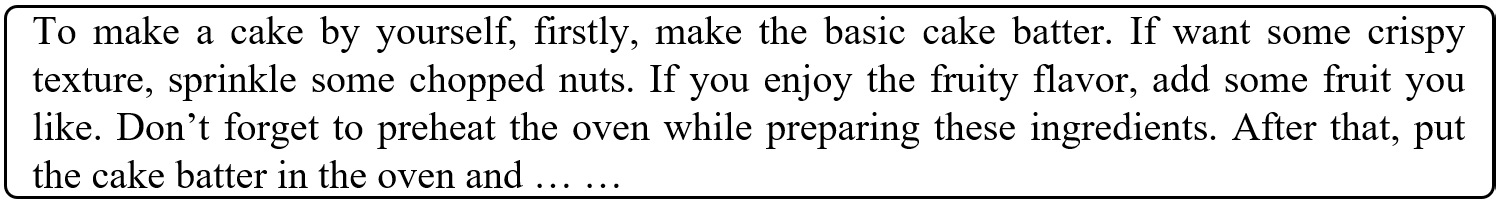
\includegraphics[width=\linewidth]{figures/appendix/Case_text.png}\label{fig:Case_text}}
    \vspace{0cm}
    \subfigure[Screenshot of the procedural graph extracted by PET]{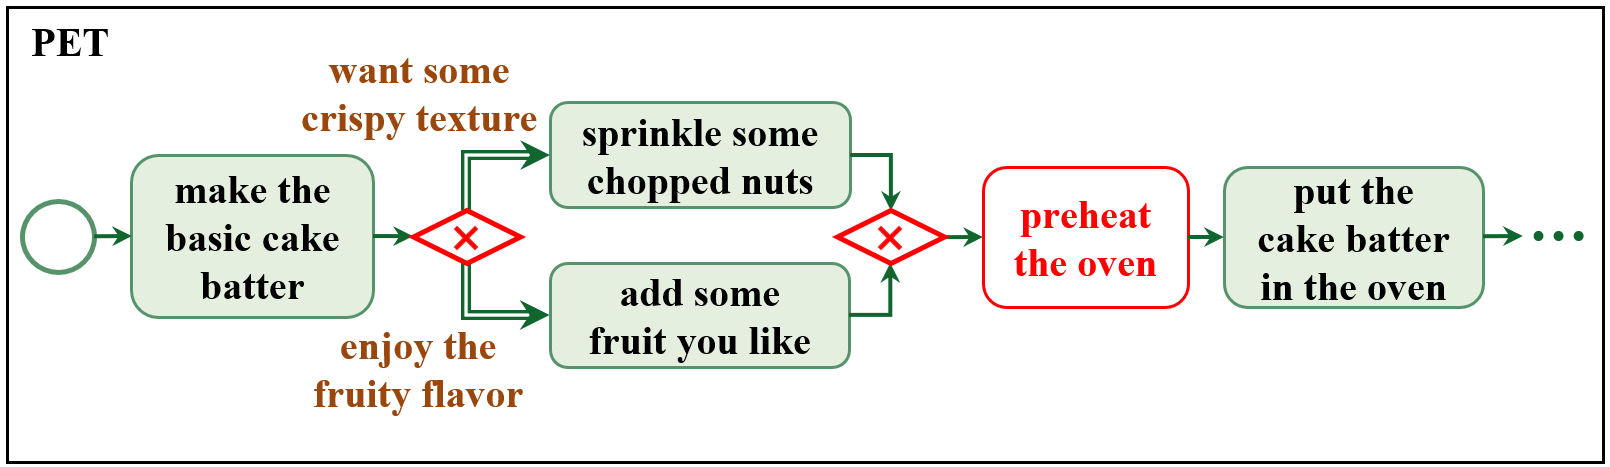
\includegraphics[width=\linewidth]{figures/appendix/Case_pet.png}\label{fig:Case_pet}}
    \vspace{0cm}
    \subfigure[Screenshot of the procedural graph extracted by fine-tuned Llama2]{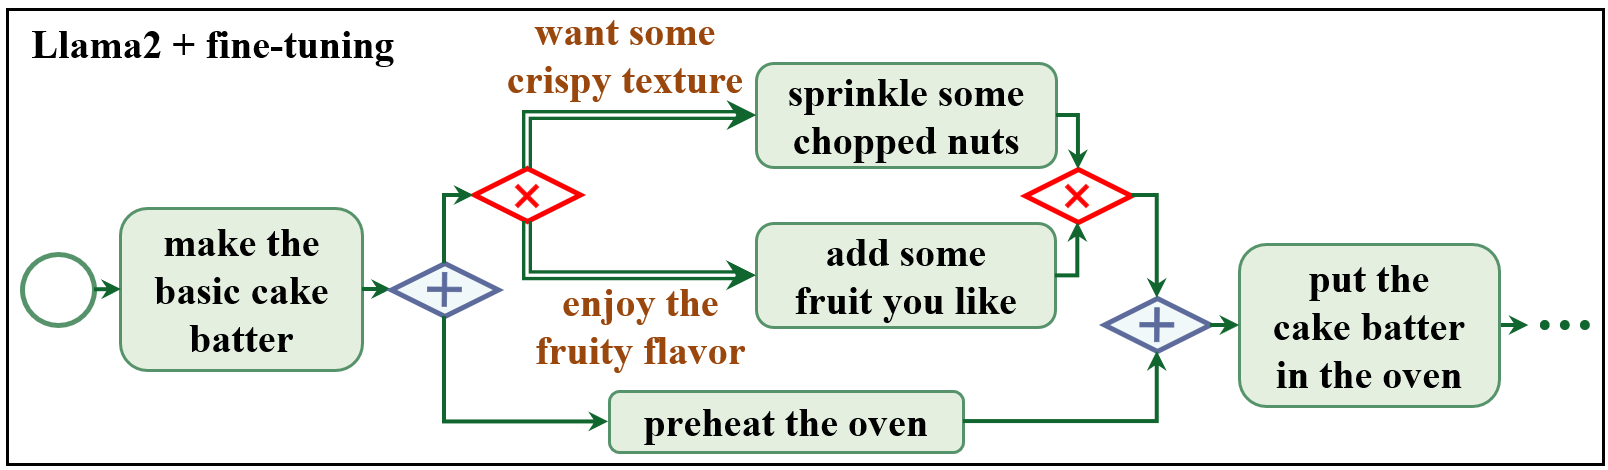
\includegraphics[width=\linewidth]{figures/appendix/Case_tuning.png}\label{fig:Case_tuning}}
    \vspace{0cm}
    \subfigure[Screenshot of the procedural graph extracted by fine-tuned Llama2 with self-refine strategy]{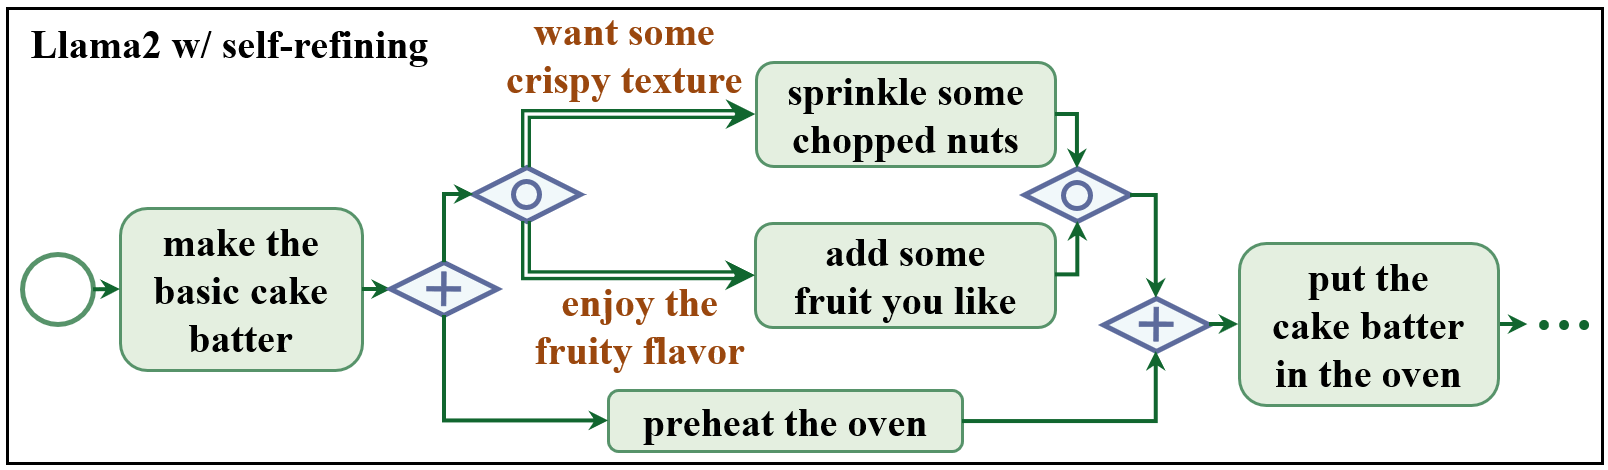
\includegraphics[width=\linewidth]{figures/appendix/Case_self.png}\label{fig:Case_self}}

    \zsavepos{figure-2}

    \zsavepos{figure-2}
    \zsavepos{figurecap-1}
    \zsavepos{figurecap-1}\caption{Illustration of case study.
    }\zsavepos{figurecap-2}\zsavepos{figurecap-2}
    \label{fig:case_study}
    \zlabel{figure}

    \zlabel{figure}
\end{figure}

\phantom{Invisible Text}
\vspace{-\baselineskip}

\zsavepos{header-1}

\zsavepos{header-1}\subsection{Case Study\zsavepos{header-2\zsavepos{header-2}}
\zsavepos{header-3}\zlabel{header}
}\zsavepos{header-3}\zlabel{header}

As shown in Figure~\ref{fig:case_study}, PET~\ref{fig:Case_pet} fails to handle the parallel actions in the document~\ref{fig:Case_text} due to the lack of the ability to understand complex expressions, and it uses the wrong type of gateway to organize the non-sequential actions ``sprinkle some chopped nuts'' and ``add some fruit you like'' as it can only deal with partial types of gateways. Fine-tuned Llama2~\ref{fig:Case_tuning} successfully organizes the parallel execution of actions in the document, but also uses the wrong gateway to organize the non-sequential actions ``sprinkle some chopped nuts'' and ``add some fruit you like''. With the help of our designed verifier~\ref{fig:Case_self}, fine-tuned Llama2 with self-refine strategy correct the wrong gateway into inclusive gateway through the feedback provided by the verifier, as there exists no conflict between the conditions ``want some crispy texture'' and ``enjoy the fruity flavor''. This demonstrates the effectiveness of our proposed strategy by paying extra attention to non-sequential logic prediction.

\begin{figure*}[th]
    \zsavepos{figure*-1}
    \zsavepos{figure*-1}
    \centering
    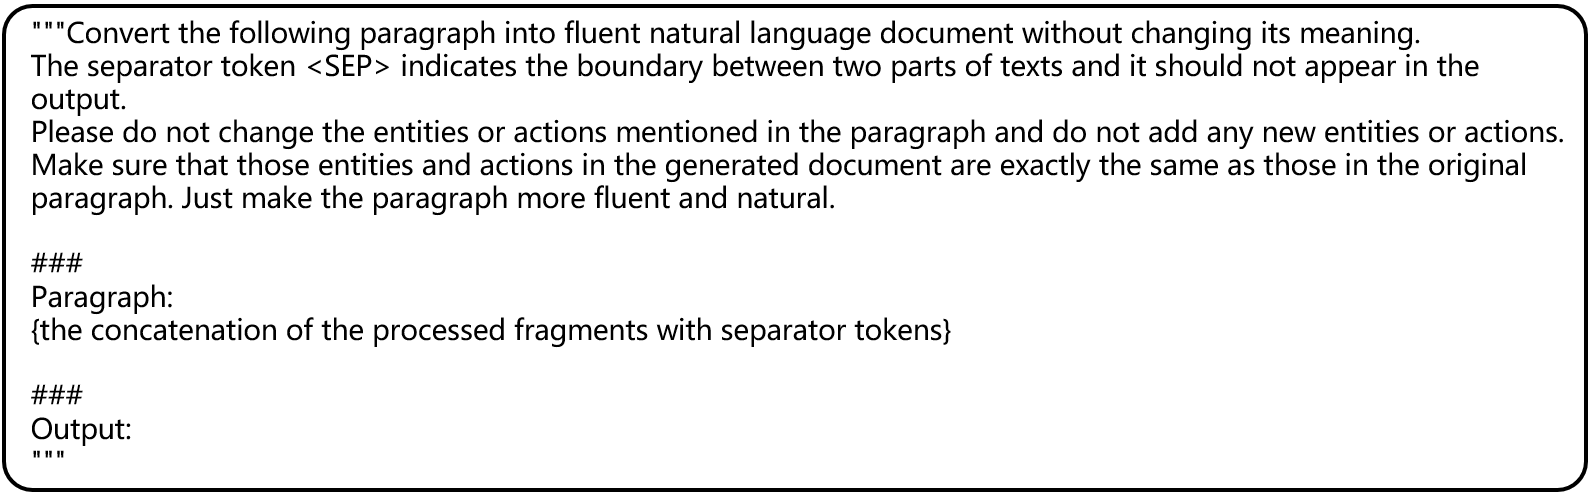
\includegraphics[width=\textwidth]{figures/prompt/Rephrase.png}
    \zsavepos{figure*-2}

    \zsavepos{figure*-2}
    \zsavepos{figurecap*-1}
    \zsavepos{figurecap*-1}\caption{The designed prompt used to rephrase the concatenation of the processed fragments.
    }\zsavepos{figurecap*-2}\zsavepos{figurecap*-2}
    \label{fig:Rephrase}
    \vspace*{-0cm}
    \zlabel{figure*}

    \zlabel{figure*}
\end{figure*}

\begin{figure*}[!th]
    \zsavepos{figure*-1}
    \zsavepos{figure*-1}
    \centering
    \subfigure[Template for inclusive gateway refinement]{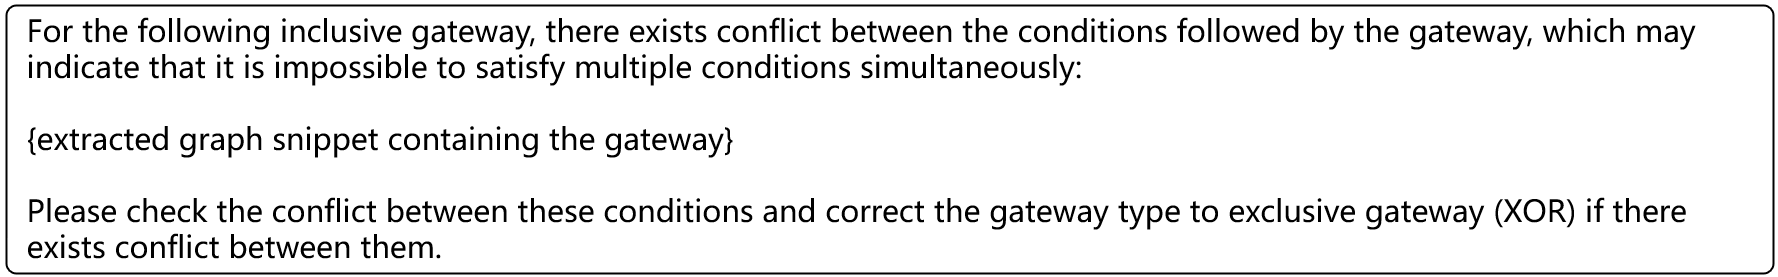
\includegraphics[width=1\textwidth]{figures/appendix/OR_verifier.png}\label{fig:verifier_or}}
    \vspace{0cm}
    \subfigure[Template for exclusive gateway refinement]{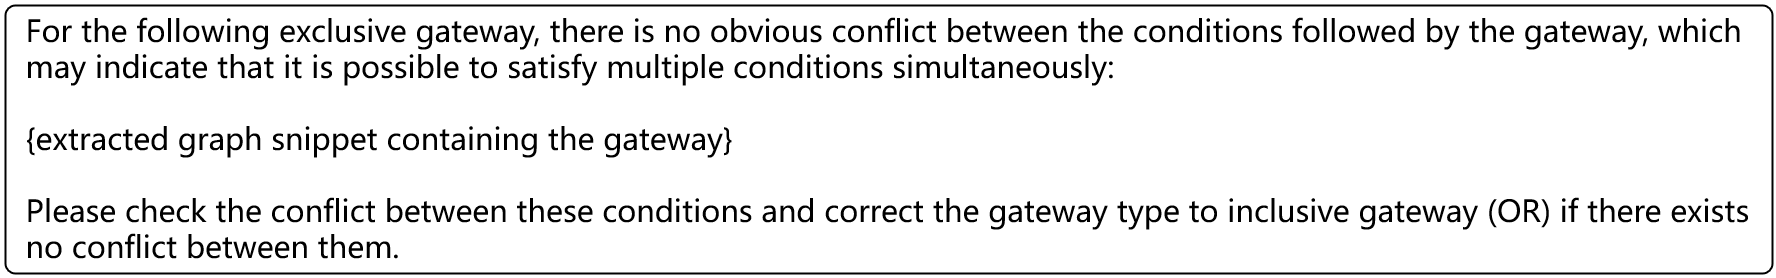
\includegraphics[width=1\textwidth]{figures/appendix/XOR_verifier.png}\label{fig:verifier_xor}}
    \vspace{0cm}
    \subfigure[Template for parallel gateway refinement]{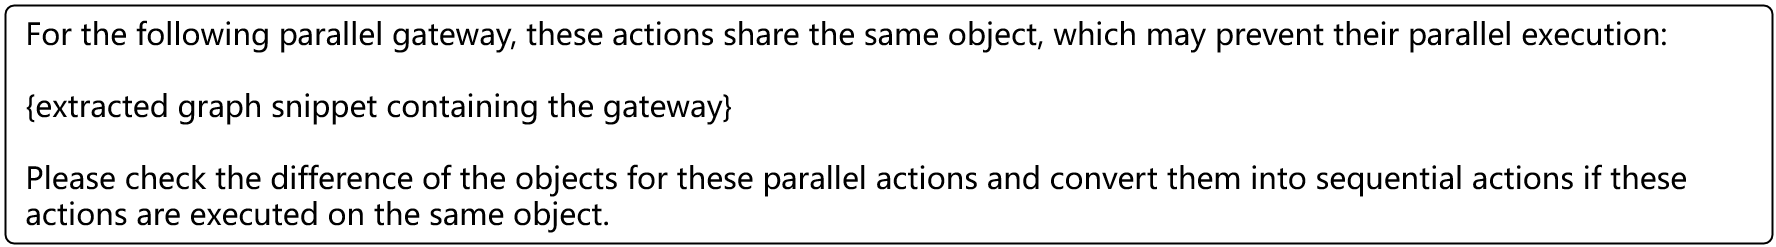
\includegraphics[width=1\textwidth]{figures/appendix/Parallel_verifier.png}\label{fig:verifier_parallel}}
    \vspace{0cm}
    \subfigure[Template for sequential actions refinement]{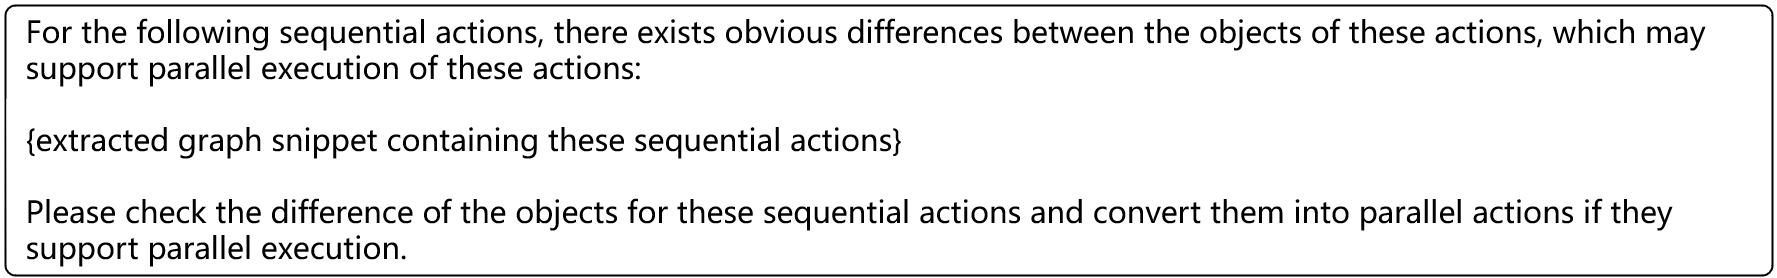
\includegraphics[width=1\textwidth]{figures/appendix/Sequential_verifier.png}\label{fig:verifier_sequential}}

    \zsavepos{figure*-2}

    \zsavepos{figure*-2}
    \zsavepos{figurecap*-1}
    \zsavepos{figurecap*-1}\caption{Designed templates of our proposed verifiers.
    }\zsavepos{figurecap*-2}\zsavepos{figurecap*-2}
    \label{fig:verifier}
    \zlabel{figure*}

    \zlabel{figure*}
\end{figure*}

\begin{figure*}[t]
    \zsavepos{figure*-1}
    \zsavepos{figure*-1}
\ContinuedFloat
    \centering
    \subfigure{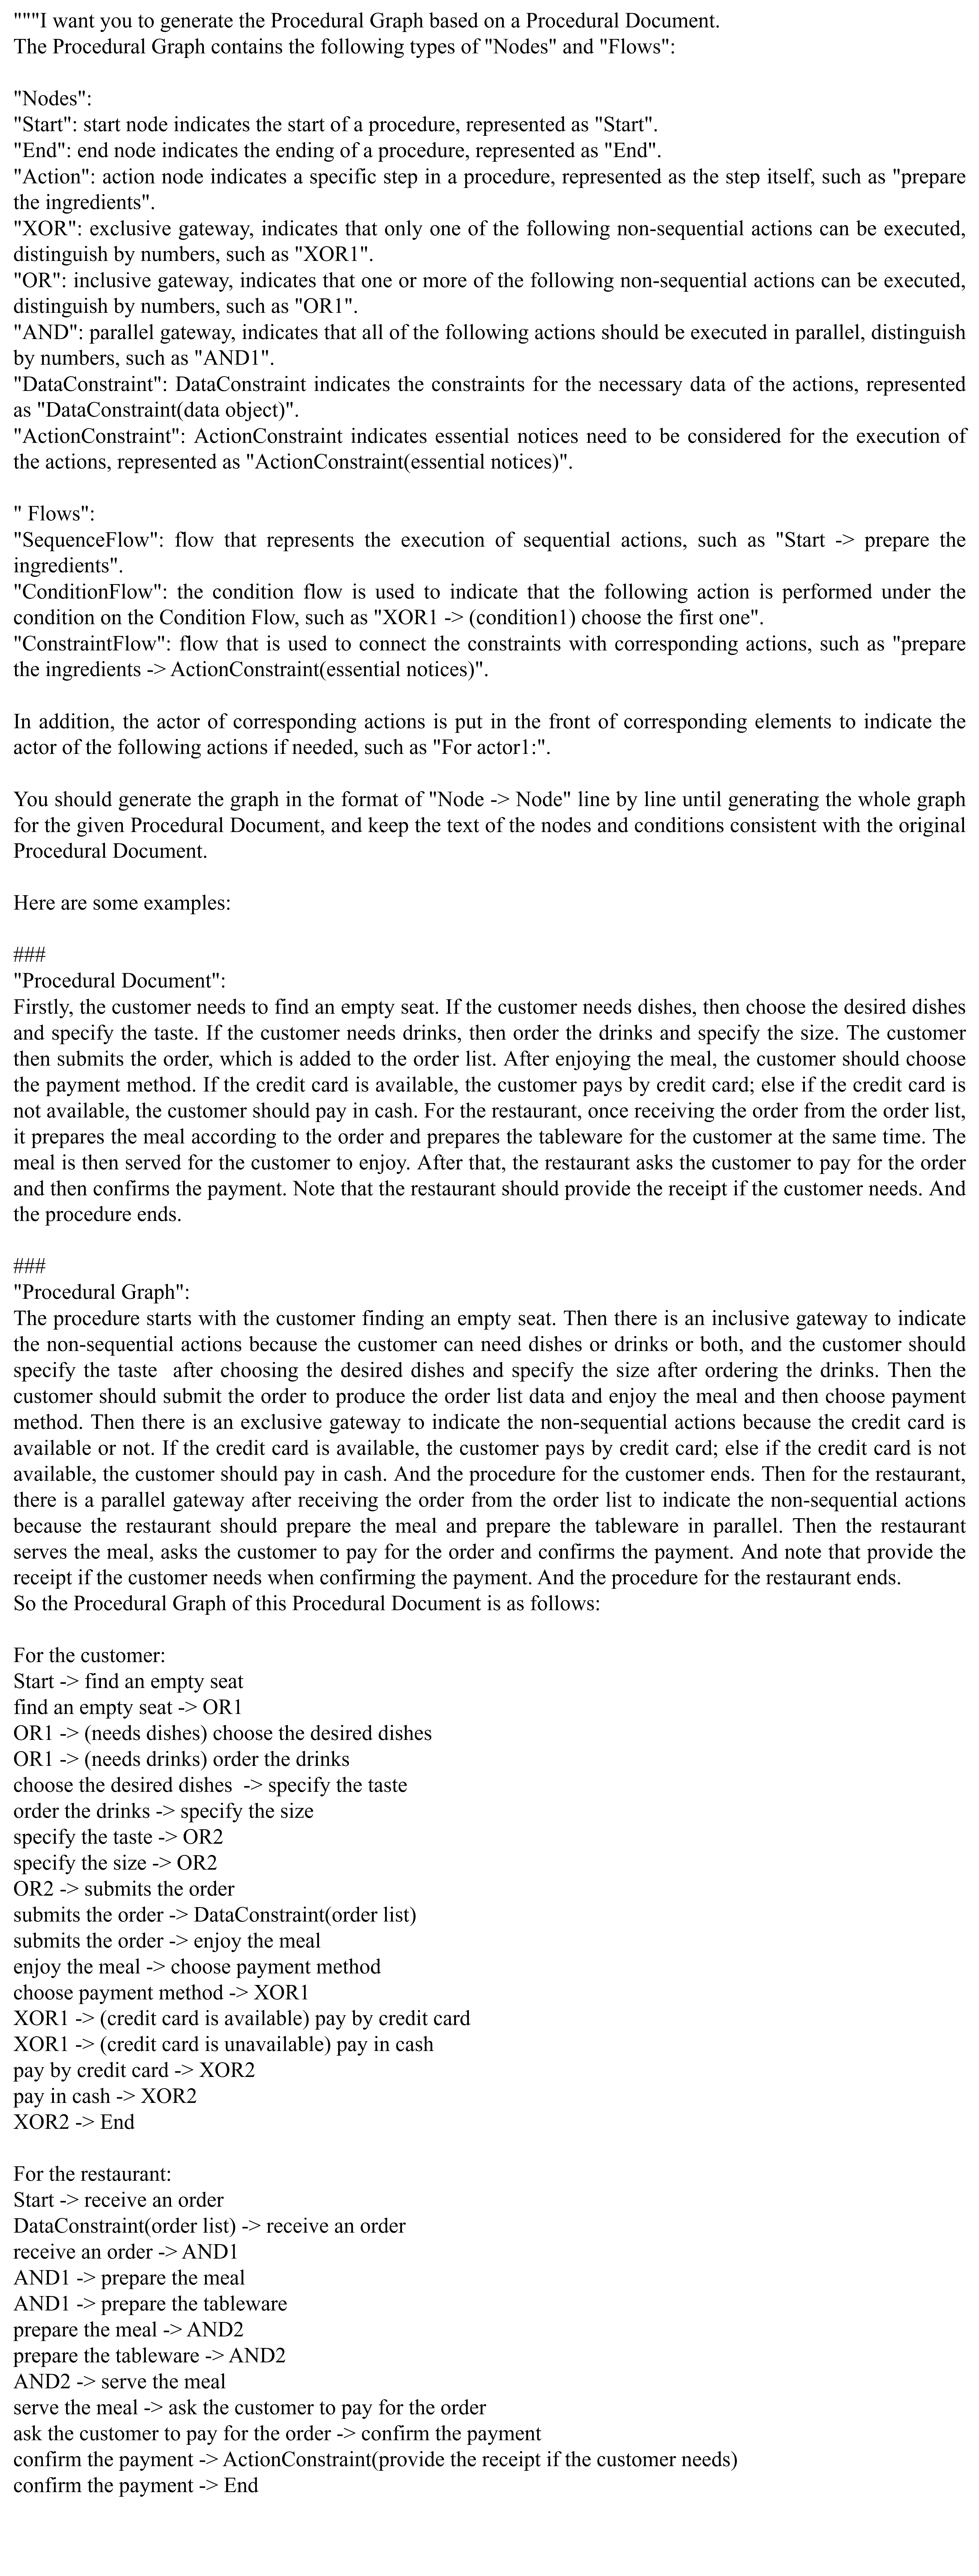
\includegraphics[width=0.48\textwidth]{figures/prompt/Prompt1.png}
    \zsavepos{figure*-2}

    \zsavepos{figure*-2}
\label{fig:Prompt1}}\vspace{-0.3cm}
    \subfigure{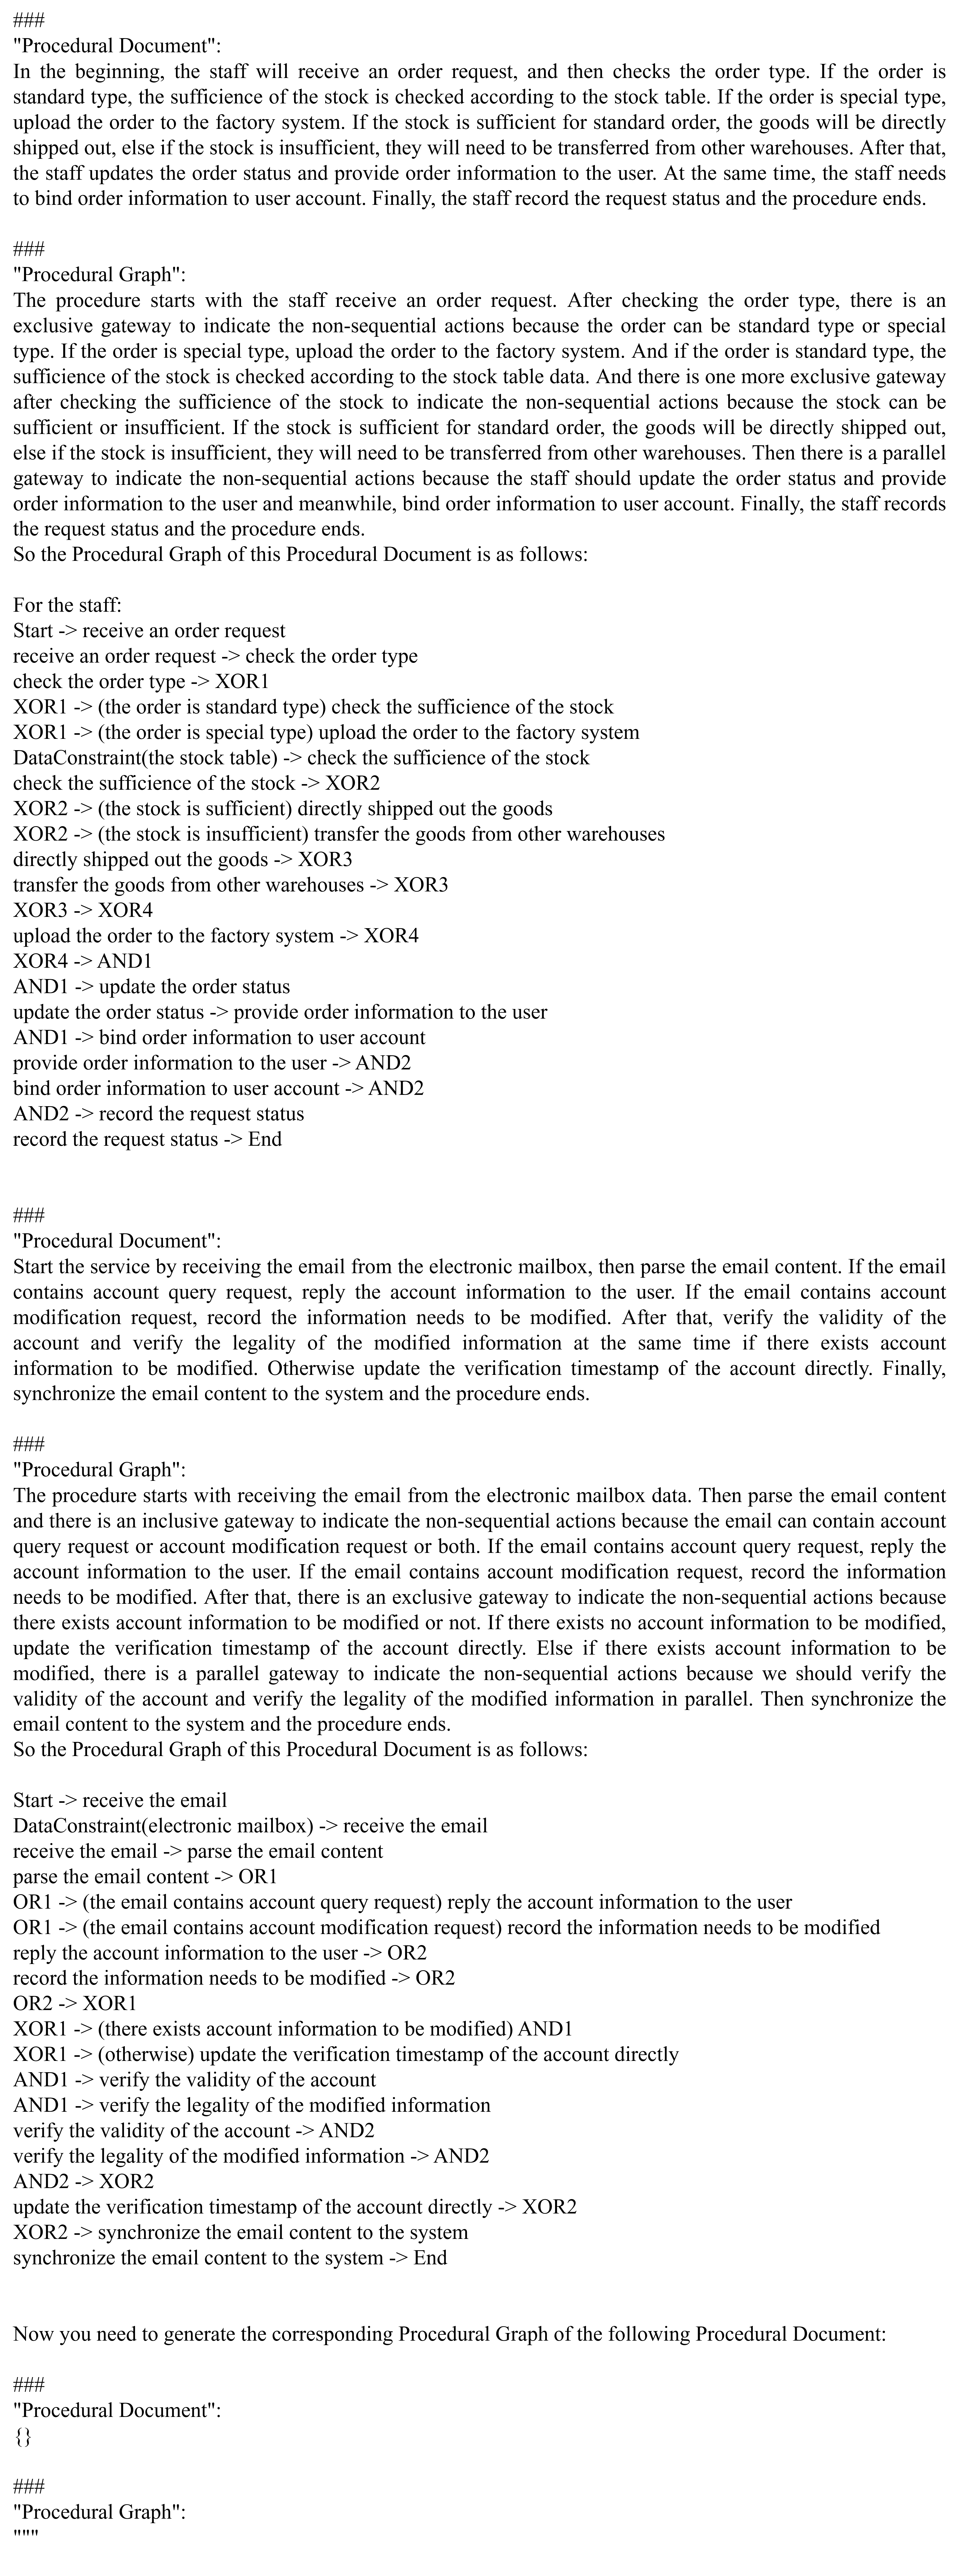
\includegraphics[width=0.48\textwidth]{figures/prompt/Prompt2.png}\label{fig:Prompt2}}
    \zsavepos{figurecap*-1}
    \zsavepos{figurecap*-1}\caption{The adopted prompt consisting of elaborate instruction and three examples.
    }\zsavepos{figurecap*-2}\zsavepos{figurecap*-2}
    \label{fig:GenerationPrompt}
    \zlabel{figure*}

    \zlabel{figure*}
\end{figure*}
